\documentclass[a4paper, openany]{memoir}

\usepackage[utf8]{inputenc}
\usepackage[T1]{fontenc} 
\usepackage[english]{babel}
\usepackage{amsmath}
\usepackage{amssymb}

\usepackage{booktabs}
\usepackage{fancyhdr}
\usepackage{float}
\usepackage{indentfirst}
\usepackage{graphicx}
\usepackage[linewidth=1pt]{mdframed}
\usepackage{multicol}
\usepackage{fancyvrb}

\pagestyle{fancy}
\fancyhf{}
\fancyhead[LE]{\leftmark}
\fancyhead[RO]{\rightmark}
\fancyhead[RE, LO]{PSD}
\fancyfoot[LE, RO]{\thepage}
\fancyfoot[RE, LO]{Pete Gautam}

\renewcommand{\headrulewidth}{1.5pt}

\chapterstyle{thatcher}
\setcounter{chapter}{2}

\begin{document}

\chapter{Change Management}
\section{Why change management}
Assume that we have 2 people working on the same code base, as shown below:
\begin{figure}[H]
    \centering
    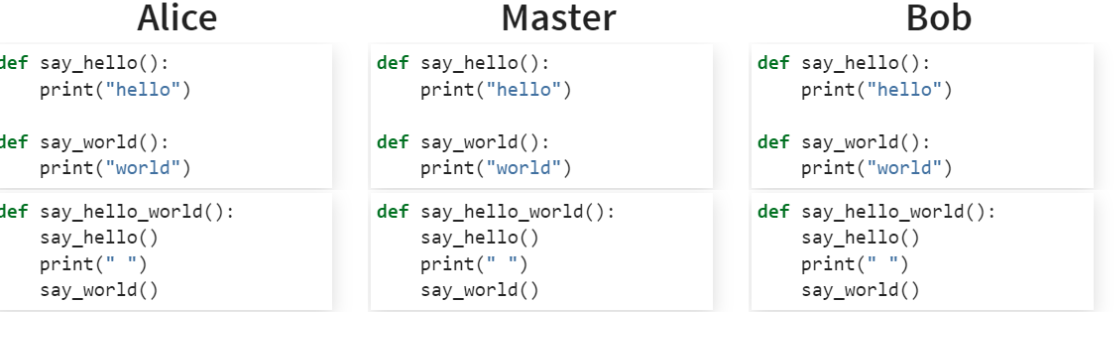
\includegraphics[scale=0.5]{src/3.1 Example1.PNG}
\end{figure}
\noindent The master version of the code is the final, centralised version that combines both Alice and Bob's work. Then, Alice refactors code (makes the code simpler), and Bob extends code.
\begin{figure}[H]
    \centering
    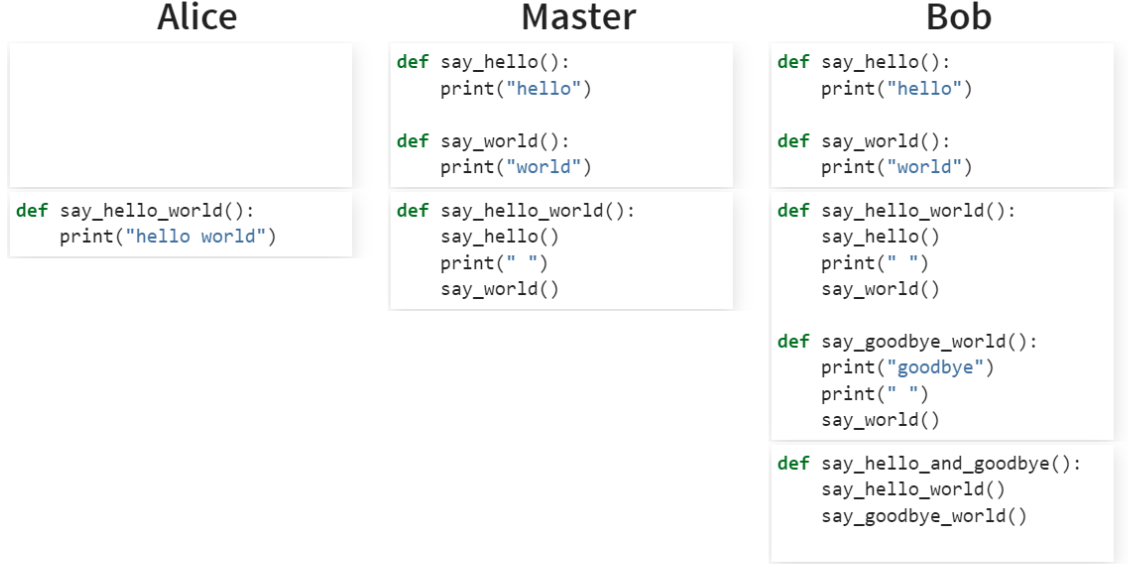
\includegraphics[scale=0.5]{src/3.2 Example2.PNG}
\end{figure}
Now, Alice and Bob both want to update the master version of the code. If Alice copies first to master then Bob, we end up at the following state.
\begin{figure}[H]
    \centering
    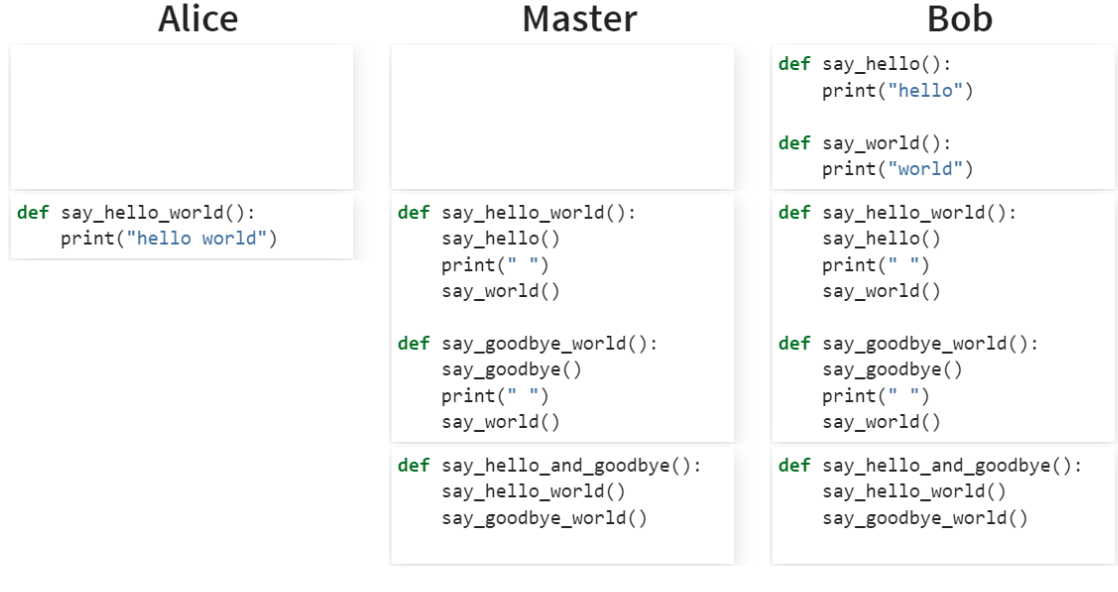
\includegraphics[scale=0.5]{src/3.3 Example3.PNG}
\end{figure}
\noindent In this case, Alice has wiped the first file, but Bob overrides the second file- the function \texttt{say\_hello\_world} does not work since \texttt{say\_hello} and \texttt{say\_world} have gone missing. So, the code is broken. 

Instead, if Bob copies first to master then Alice, we end up at the following state.
\begin{figure}[H]
    \centering
    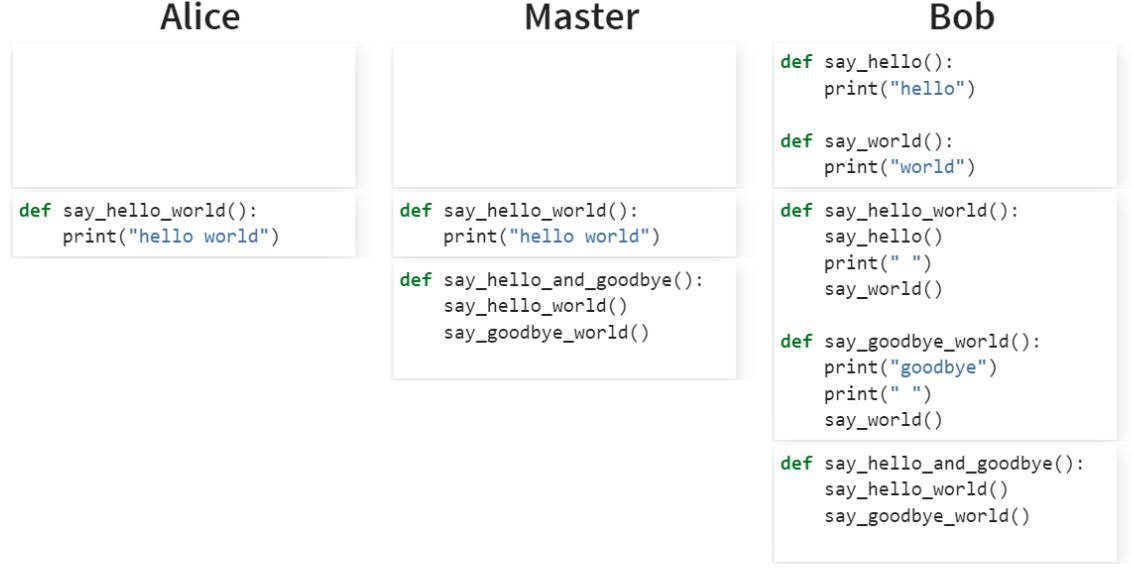
\includegraphics[scale=0.5]{src/3.4 Example4.PNG}
\end{figure}
\noindent In this case as well, Alice still wipes the first file, meaning that the new file doesn't compile- the function \texttt{say\_hello\_and\_goodbye} does not work since \texttt{say\_goodbye\_world} has gone missing. So, the code is broken.

So, it doesn't matter who compiles first- the code still breaks after the changes get made. This is why we need a change management system. Without careful change management, there is no way of knowing what version of the constantly changing code base has been used during the process.

For example, the results from code testing is useless without code management. It is not possible to tell what version the report applies to. Moreover, the code might have already been changed/bugs fixed since it was test. This also applies to:
\begin{itemize}
    \item compilation,
    \item dependency management,
    \item code reviews,
    \item static analysis,
    \item refactoring,
    \item deployment and rollback,
    \item bug reporting and triage.
\end{itemize}

\section{What are change control items}
Any item that is directly edited by the team is a change control item, e.g.
\begin{itemize}
    \item source code files,
    \item build scripts or configuration files,
    \item default application configuration files,
    \item user documentation,
    \item requirements specification,
    \item version control tool configurations, etc.
\end{itemize}
Anything indirectly generated by the manually edited files are not change control items, and should not be committed to the version control system, e.g.
\begin{itemize}
    \item compiled binaries,
    \item third party libraries,
    \item compiled document formats, e.g. PDF, PS,
    \item auto-generated source code files,
    \item client side IDE configuration,
    \item log files, etc.
\end{itemize}

Some people argue that we should store non-control items in a SCM (source code management), since:
\begin{itemize}
    \item the source code takes a long time to compile- storing cached binaries will make this faster.
    \item compilations cannot be automated- someone has to press a button on the GUI.
    \item third party libraries aren't available in a public release repository.
\end{itemize}
These are bad reasons to store non-control items in the repository. It is not a file storage system. In fact, we can solve these issues using release and dependency management. For example,
\begin{itemize}
    \item we can break code into smaller modules with separate compilation pipe-lines. Each module can be compiled easily and in parallel.
    \item agree and configure a release management process for each module using a release repository. This can depend on libraries provided by others, and also publish the ones developed by the team.
\end{itemize}

\section{Version Control System}
A version control system (e.g. git) is a centralised repository that the team can access to and make changes. This allows us to control change concurrently. The team can make changes to a working copy of the code from the centralised repository. When a member is ready to commit, they check if the repository has been updated. They receive changes from the repository and resolve any conflicts that emerged. They repeat this step until there is no change made to the repository since the last pull. At that point, they commit/push the change to the repository. A simple representation of this is given below.
\begin{figure}[H]
    \centering
    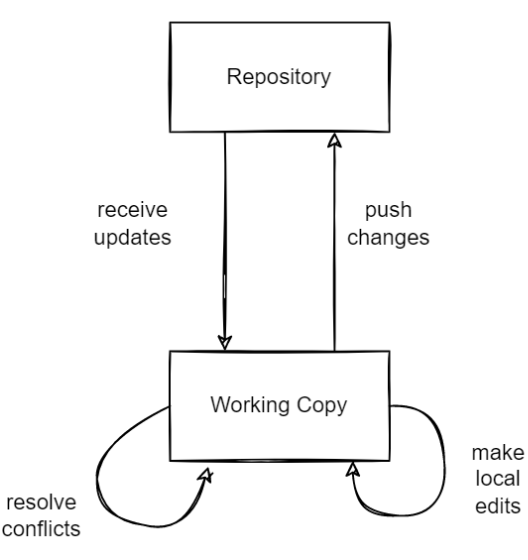
\includegraphics[scale=0.6]{src/3.5 VCS.png}
    \caption{The workflow in a version control system}
\end{figure}

A change control system can be centralised or distributed:
\begin{itemize}
    \item In a centralised version control system, there is one single centralised repository on the server. Everyone has working copies on their machine, which they can use to push their code to the repository. The following figure summarises this.
    \begin{figure}[H]
        \centering
        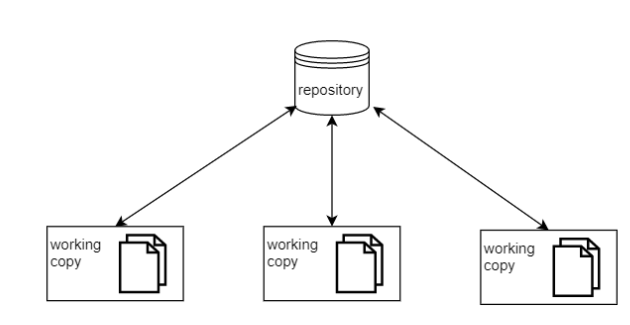
\includegraphics[scale=0.65]{src/3.8 Centalised.png}
        \caption{A centralised version controlled system}
    \end{figure}

    \item In a distributed version control system, there are multiple repositories. Every developer has a local repository. They can check out a working copy and work on it. Changes from the local repository can be pushed/pulled from other repositories amongst the team (like peer-to-peer distribution). So, each member has a local repository and they can push from each other's repository across the network. The following figure summarises this.
    \begin{figure}[H]
        \centering
        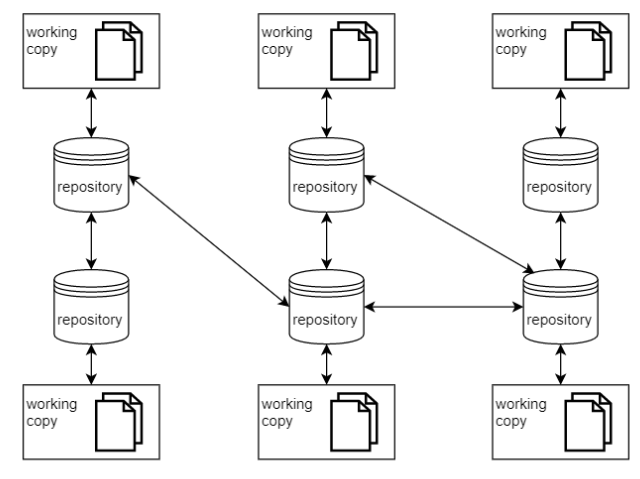
\includegraphics[scale=0.6]{src/3.6 Distributed.png}
        \caption{A distributed version controlled system}
    \end{figure}
\end{itemize}

In practice, it is quite difficult to support distributed version control system. Instead, most version control systems are hybrid- they have a centralised arrangement in a distributed fashion. So, each member has a local repository, and there is a central external repository. The team works on a local copy of the repository, and synchronise with the centralised, external repository. The following figure summarises this.
\begin{figure}[H]
    \centering
    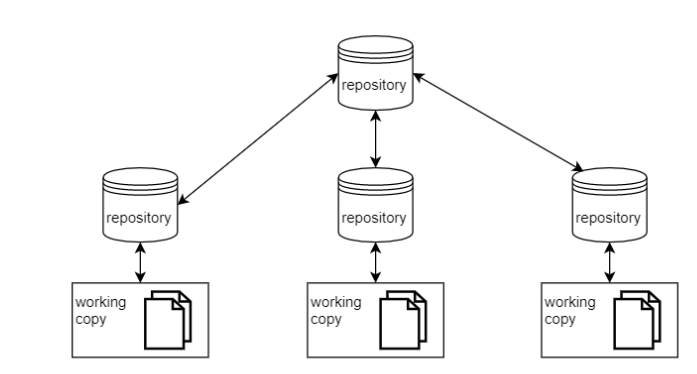
\includegraphics[scale=0.65]{src/3.7 In practice.png}
    \caption{A hybrid version controlled system}
\end{figure}

\section{Commits}
Commits can be thought of as either a package of information needed to describe the change since the previous commit, or the complete snapshot of source code at a time. Both views are equivalent.

A commit has:
\begin{itemize}
    \item a unique id;
    \item the id of the parent commit(s), to identify what code has been changed;
    \item changes to existing control items;
    \item any added/removed change control items;
    \item metadata, e.g. author, timestamp, and log message.
\end{itemize}

To produce the commit id, we can use a counter in a centralised version control system. However, this is not possible in distributed systems. Instead, they use a one-way hash function that combines all the information in a commit (i.e. previous commit ids, metadata, etc.) to produce a fixed-length id. There is a very low probability that two commits will get the same id.

The commit log message should:
\begin{itemize}
    \item have a short, meaningful title;
    \item describe the intent of the commit;
    \item link to the issue in the project tracker or the merge request;
    \item explain how the commit addresses the issue.
\end{itemize}
The message does not need to explain what code was changed- we can see that from the files changed. It does however need to explain why and how the code was changed. An example of a commit message is given below.
\begin{figure}[H]
    \centering
    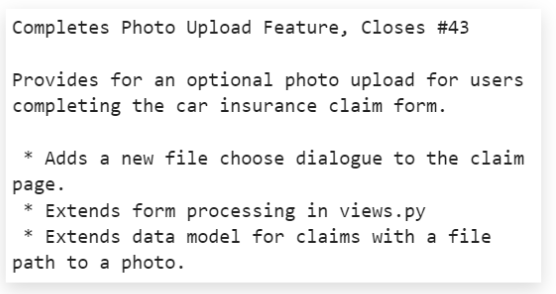
\includegraphics[scale=0.7]{src/3.11 CommitExample.PNG}
    \caption{A commit message.}
\end{figure}


\section{Branches}
Branching is the practice of maintaining multiple development lines based on a common history within a single version control repository. A commit has one parent; but the parent can have multiple children commits, all of which will be part of different branches. We can have multiple branches of concurrent development in parallel versions of the repository. It is useful for:
\begin{itemize}
    \item experimenting with implementation of new features- it may take several commits to implement this feature, and it may not work the first time round.
    \item undertaking a substantial reorganisation- experiment a big reorganisation of the repository without disrupting others' work. This version of the repository might be adopted later.
    \item supporting a specialised variant to an application- some version of the code may always be different. We maintain this variant out of the main branch.
    \item creation of a release- this is a branch where no more features are added, and we only resolve bugs. This allows us to keep adding features to the main branch (which will be part of a future release).
\end{itemize}
Different branching practices can be combined into a branching strategy for a project/team.

There are 3 main types of branching:
\begin{itemize}
    \item Trunk-based development. In this case, there is only one branch (called main, master, or trunk). The developers commit to that single branch. 
    
    This is summarised in the image below.
    \begin{figure}[H]
        \centering
        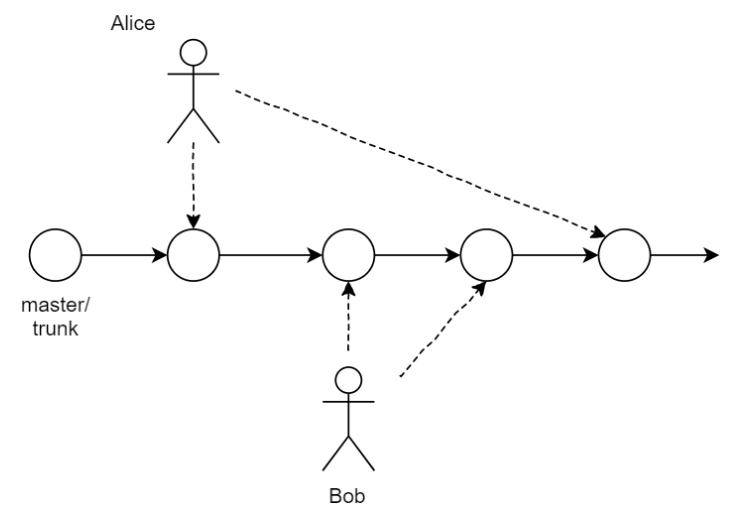
\includegraphics[scale=0.6]{src/3.9 Trunk based.png}
        \caption{Trunk-based development}
    \end{figure}
    The advantages of this approach is:
    \begin{itemize}
        \item the workflow is simple;
        \item everyone can see the current state of the project easily;
        \item it forces developers to break changes into small increments of change; and
        \item it reduces the risk of merge conflicts.
    \end{itemize}
    A disadvantage of this approach is there is a higher risk of broken code- a commit can have broken tests/broken continuous integration pipelines.
    
    \item Feature branching. In this case, there is one branch for each feature. There is a master branch. The team works on different features over different periods in different branches. This allows for concurrent development with the master branch. So, there are more frequent commits to the features branches. When features are ready, we first merge the master branch to the feature branch, and then merge the feature branch to the master branch.
    
    The advantages of this approach is:
    \begin{itemize}
        \item the team can develop features in isolation; and
        \item it is more convenient to perform code reviews.
    \end{itemize}
    A disadvantage of this approach is that this can encourage longer periods between integration.

    This is summarised in the image below.
    \begin{figure}[H]
        \centering
        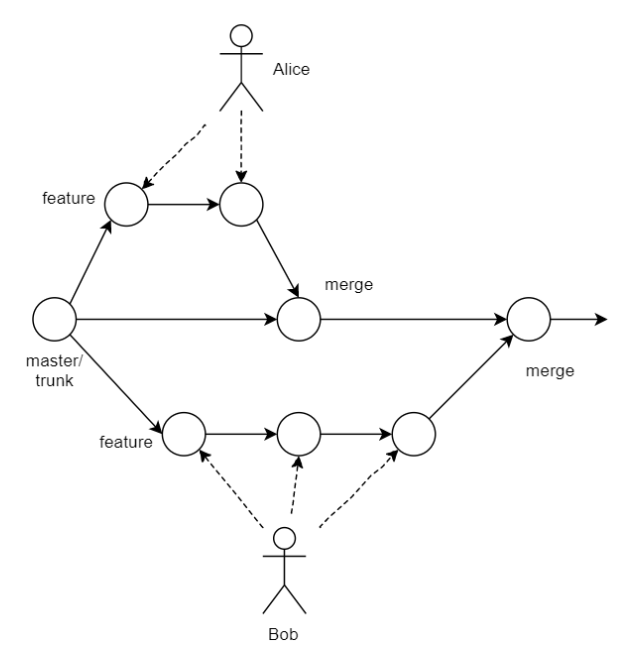
\includegraphics[scale=0.6]{src/3.10 Feature branching.PNG}
        \caption{Feature branching development}
    \end{figure}
    

    \item Staging branching. In this case, there is a branch that runs parallel to the master branch. This is different to feature branches, which are temporary. This allows changes that have been committed to spend some time in a UAT (user-acceptance testing) environment. Then, it gets merged to the master branch after user testing. In contemporary software development, some teams configure UAT environment for each feature branch- this combines both staging and feature branching. The following image summarises this approach.
    \begin{figure}[H]
        \centering
        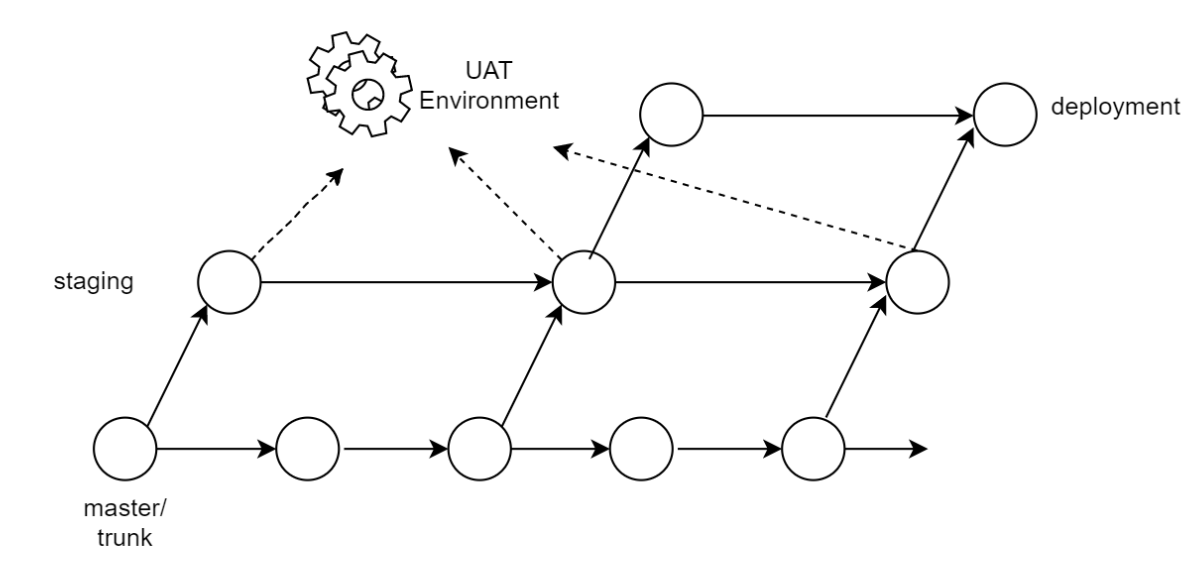
\includegraphics[scale=0.45]{src/3.8 Staging branches.png}
        \caption{Staging branching development}
    \end{figure}
\end{itemize}

When naming branches, we should following conventions to enhance project maintainability. For example, the main branch of the repository is called the master/trunk branch. It contains the primary version of the project. The user acceptance testing branch can be called staging, UAT or preprod(uction). Similarly, the production branch can be called deploy(ment) or prod(uction). When naming feature branches, we can follow a hierarchical approach, e.g. feature/webapp/splash.

In a software development project, a team follows a collection of (often customised) branching practices. There are many standard published branching strategies, e.g. Gitflow, Github flow. Most teams tailor their strategy to suit their circumstances.

It is common to manage branch growth. It is a good idea to delete branches after there is no further use to it. Also, commits can be squashed- we can merge all commits on a feature branch into one commit before merging the branch itself to the main branch.

In summary, disciplined change management, supported by an automated version control system, is fundamental to software engineering.


\end{document}